\chapter{Quantum Mechanics}

\textit{The solution of the difficulty is that the two mental pictures which experiment lead us to form - the one of the particles, the other of the waves - are both incomplete and have only the validity of analogies which are accurate only in limiting cases.}\\
\noindent\textbf{-   Werner Heisenberg}

\vspace{0.5cm}

\begin{marginfigure}[-130pt]
  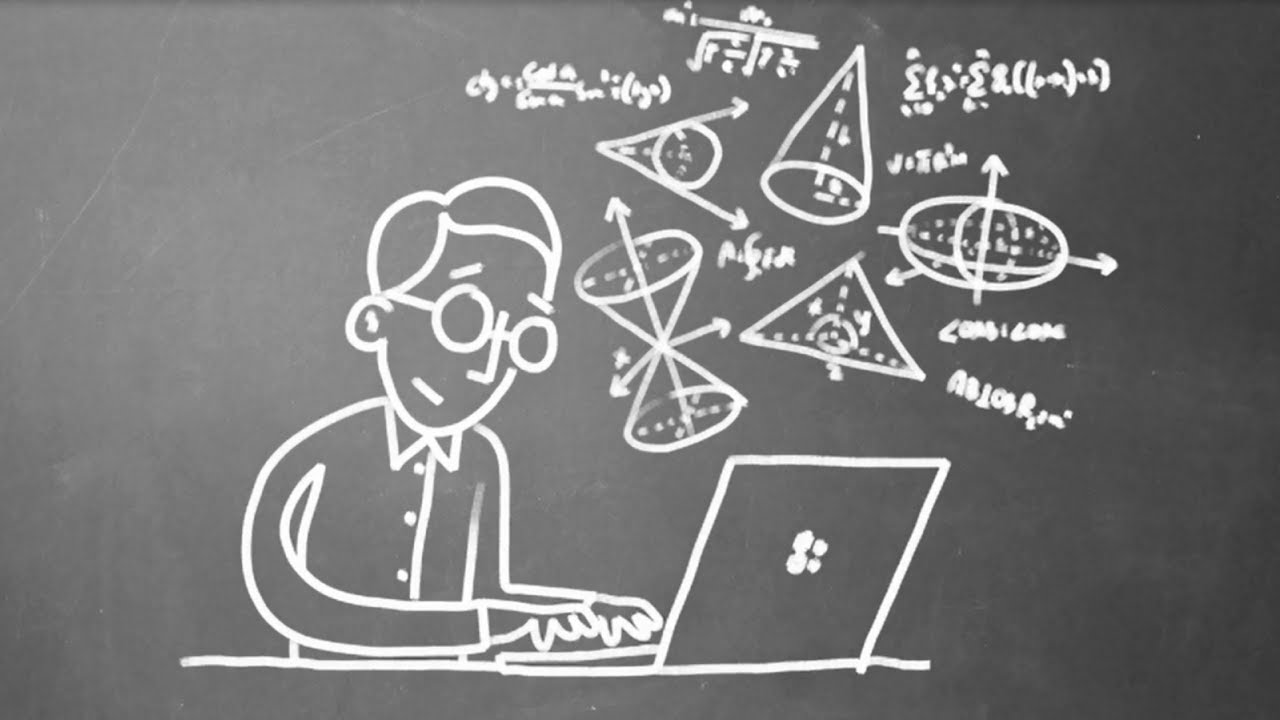
\includegraphics[width=\linewidth]{snowden.jpg}
  \caption{Snowden says NSA is building a quantum computer}
  \label{fig:marginfig}
\end{marginfigure}

A quantum (plural: quanta) is the minimum amount of any physical quantity involved in an interaction.  For example, angular momentum $J$ is quantized into units $\hbar$.
$$J_n=n\hbar$$
Quantum mechanics describes systems with probability distributions in space and time.  The probabilities describe discrete particle events.  The structure of those distributions however have wavelike features.  This is known as wave particle duality.
Quantum mechanics gradually arose from Max Planck's solution in 1900 to the black-body radiation problem and Albert Einstein's 1905 paper which offered a quantum-based theory to explain the photoelectric effect (reported 1887). 

\section{Blackbody Radiation}
\subsection{Rayleigh-Jeans Law (Classical)}
\marginnote[-260pt]{In 1900, the British physicist Lord Rayleigh derived the $\lambda^{-4}$ dependence of the Rayleigh-Jeans law based on classical physical arguments and empirical facts.  The proportionality constant was added by Rayleigh and Sir James Jeans in 1905. The Rayleigh-Jeans law revealed an important error in physics theory of the time as it predicted an energy output that diverges towards infinity as wavelength approaches zero and energy output at short wavelengths disagreed with this prediction.
This was known as the ultraviolet catastrophe.  The term "ultraviolet catastrophe" was first used in 1911 by Paul Ehrenfest, but the concept originated with the 1900 derivation of the Rayleigh-Jeans law. The phrase refers to the fact that the Rayleigh-Jeans law accurately predicts experimental results at radiative frequencies below 105 GHz, but begins to diverge with empirical observations as these frequencies reach the ultraviolet region of the electromagnetic spectrum}
\begin{marginfigure}[10pt]
  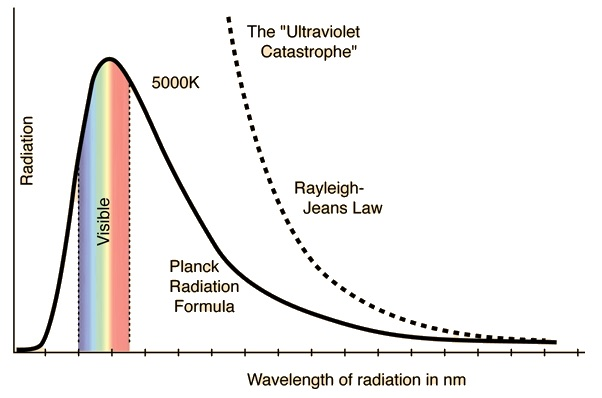
\includegraphics[width=\linewidth]{raleigh.jpg}
  \caption{Ultraviolet catastrophe}
  \label{fig:marginfig}
\end{marginfigure}
The Rayleigh-Jeans law attempts to describe the spectral radiance of electromagnetic radiation at all wavelengths from a black body at a given temperature through classical arguments.
$$I(\lambda,T)=\frac{2\pi c k_B T}{\lambda^4}$$
In 1838, Michael Faraday discovered cathode rays. By 1859 the black-body radiation problem had been identified by Gustav Kirchhoff. 
\subsection{Planck Spectrum (Modern)}
Ludwig Boltzmann suggested that the energy states of a physical system can be discrete in 1877 and by 1900 the quantum hypothesis had ben made by Max Planck.  The hypothesis states that energy is radiated and absorbed in discrete "quanta" (or energy elements).  Statistically this models the intensity $I$ as a particular function of wavelength and temperature.  This distribution is known as the Planck spectrum.
$$I(\lambda,T)=\frac{2\pi h c^2 }{\lambda^5\left(e^{\frac{hc}{\lambda k_B T}}-1\right)}$$
The Planck spectrum precisely matched the observed patterns of black-body radiation.  Specifically it matched Wien's displacement law.
\marginnote[-180pt]{
\begin{itemize}
  \item Molecules have discrete energy states $E_n$
  $$E_n=nhf $$
   \item Energy is released in discrete packets of electromagnetic radiation called "photons"
   $$E_{photon}=hf $$
\end{itemize}}
\begin{marginfigure}[-80pt]
  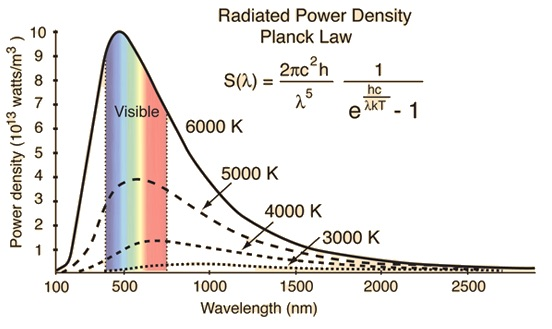
\includegraphics[width=\linewidth]{planck_spectrum.jpg}
  \caption{Planck spectrum}
  \label{fig:marginfig}
\end{marginfigure}

Wien's displacement law states that the black body radiation curve for different temperatures peaks at a wavelength inversely proportional to the temperature. 
$$\lambda_{peak}=\frac{2900\ \mu \text{m}\cdot\text{K}}{T}$$
The shift of that peak is a direct consequence of the Planck radiation law which describes the spectral brightness of black body radiation as a function of wavelength at any given temperature. However it had been discovered by Wilhelm Wien several years before Max Planck developed that more general equation, and describes the entire shift of the spectrum of black body radiation toward shorter wavelengths as temperature increases.


\begin{marginfigure}[-50pt]
  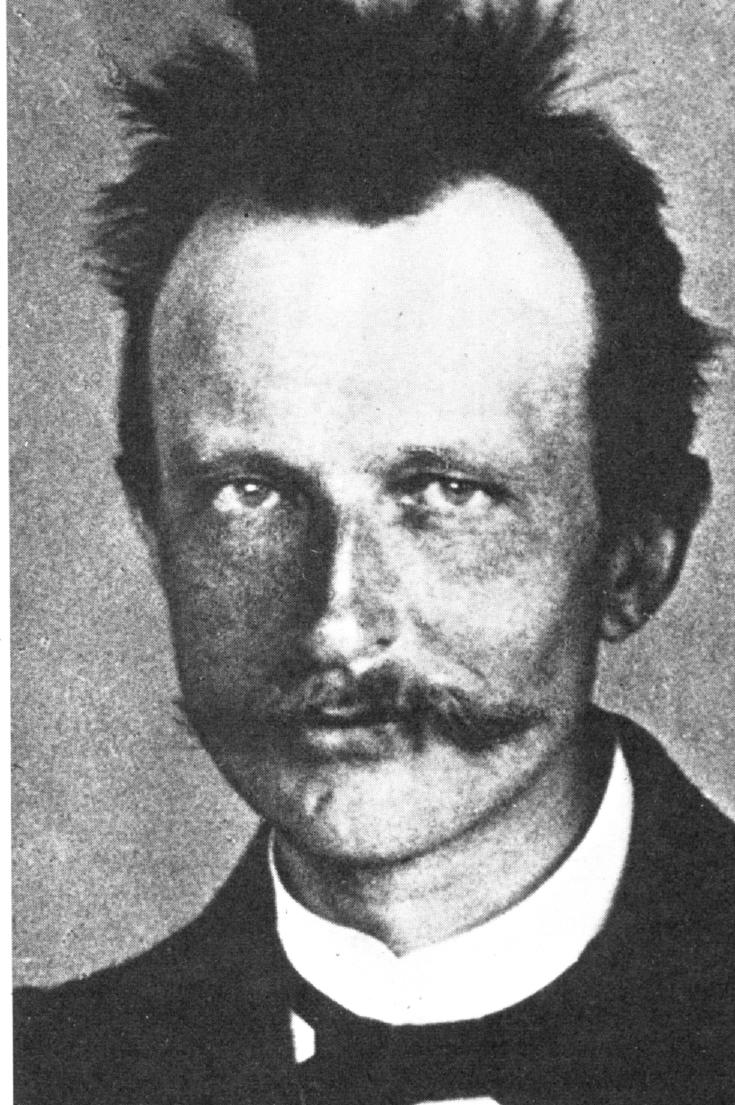
\includegraphics[width=\linewidth]{planck.jpg}
  \caption{Young Max Planck }
  \label{fig:marginfig}
\end{marginfigure}

\begin{marginfigure}[0pt]
  \includegraphics[width=\linewidth]{PE_effect.jpg}
  \caption{Photoelectric tube }
  \label{fig:marginfig}
\end{marginfigure}
\section{Photoelectric Effect}
The photoelectric effect is the observation that many metals emit electrons when light shines upon them. Electrons emitted in this manner can be called photoelectrons.  

According to classical electromagnetic theory, this effect can be attributed to the transfer of energy from the light to an electron in the metal. From this perspective, an alteration in either the intensity or wavelength of light would induce changes in the rate of emission of electrons from the metal. Furthermore, according to this theory, a sufficiently dim light would be expected to show a time lag between the initial shining of its light and the subsequent emission of an electron. However, the experimental results did not correlate with either of the two predictions made by classical theory.

Instead, electrons are only dislodged by the impingement of photons when those photons reach or exceed a threshold frequency. Below that threshold, no electrons are emitted from the metal regardless of the light intensity or the length of time of exposure to the light. To make sense of the fact that light can eject electrons even if its intensity is low, Albert Einstein proposed that a beam of light is not a wave propagating through space, but rather a collection of discrete wave packets (photons), each with energy hf. This shed light on Max Planck's previous discovery of the Planck relation (E = hf) linking energy (E) and frequency (f) as arising from quantization of energy. The factor h is known as the Planck constant.

In 1887, Heinrich Hertz discovered that electrodes illuminated with ultraviolet light create electric sparks more easily. In 1905 Albert Einstein published a paper that explained experimental data from the photoelectric effect as the result of light energy being carried in discrete quantized packets. This discovery led to the quantum revolution.
The work function $W$ is the work required to free an electron from the metal.  
\begin{marginfigure}[-80pt]
  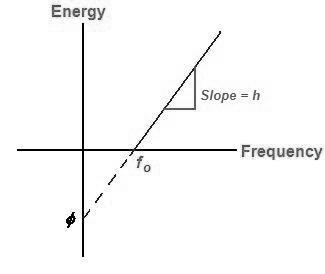
\includegraphics[width=\linewidth]{PE_graph.jpg}
  \caption{Photoelectric effect graph}
  \label{fig:marginfig}
\end{marginfigure}
$$KE_{max}=hf-W$$
$$KE_{max}=eV_{stop}$$

Electrons will not be emitted if incident light is below a certain cutoff frequency even if intensity of light is increased.  

\section{Compton Effect}
Compton scattering, discovered by Arthur Holly Compton, is the inelastic scattering of a photon by a charged particle, usually an electron.\marginnote[100pt]{ Compton scattering results in a decrease in energy (increase in wavelength) of the photon.  This is called the Compton effect. Part of the energy of the photon is transferred to the recoiling electron.  The scattering supports particle nature of light.}
$$\lambda'-\lambda_0=\frac{h}{mc}\left(1-\cos \theta\right)$$

\begin{figure}
  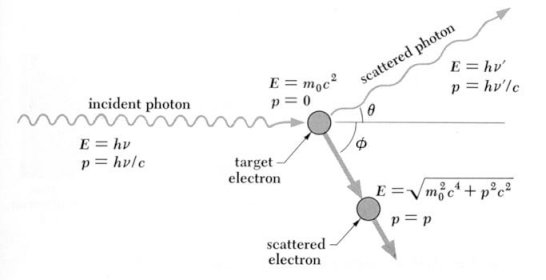
\includegraphics[width=\linewidth]{compton.jpg}
  \caption{Compton scattering}
  \label{fig:fig}
\end{figure}

\section{De Broglie Relation}\marginnote[0pt]{\subsection{Planck-Einstein Relation}
$$E=\frac{h}{T}=hf=\hbar \omega$$}
All matter can exhibit wave-like behavior. For example, a beam of electrons can be diffracted just like a beam of light or a water wave. Matter waves are a central part of the theory of quantum mechanics, being an example of wave-particle duality. The concept that matter behaves like a wave is also referred to as the de Broglie hypothesis due to having been proposed by Louis de Broglie in 1924.  Matter waves are often referred to as de Broglie waves.\\
The de Broglie wavelength is the wavelength, $\lambda$, associated with a massive particle and is related to its momentum, $p$, through the Planck constant, $h$.
$$p=\frac{h}{\lambda}=\hbar k$$
\begin{marginfigure}[0pt]
  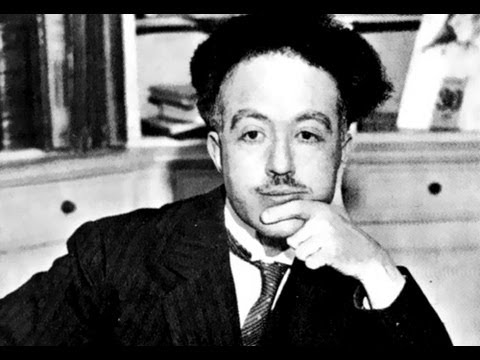
\includegraphics[width=\linewidth]{debroglie.jpg}
  \caption{Louis De Broglie}
  \label{fig:marginfig}
\end{marginfigure}
De Broglie, in his 1924 PhD thesis, proposed that just as light has both wave-like and particle-like properties, electrons also have wave-like properties.




\section{Wave functions}
\marginnote{
\subsection{Probability distributions}
For standard probability distributions average values are calculated as follows.
$$\Braket{x}=\int^\infty_{-\infty}\rho(x)x \ dx$$
$$\Braket{x^2}=\int^\infty_{-\infty}\rho(x)x^2 \ dx$$
$$\int^\infty_{-\infty}\rho(x) \ dx=1$$
} 



In quantum mechanics a wave function is a mathematical object that represents a particular pure quantum state of a specific isolated system of one or more particles. It is a central entity in quantum mechanics and provides probability distribution of states. 
$$\psi(x,t)=Ae^{-i\left(kx-\omega t\right)}=A\left( \cos \left( k x-\omega t \right)+i\sin \left( k x-\omega t \right) \right)$$
 These distributions can be used to find average values of observable quantities as follows.
$$\Braket{x}=\int^\infty_{-\infty}\psi^*(x)x\ \psi(x) \ dx$$
The wave functions provide an inner product space for a set of observable operators.  The DeBroglie relation is represented through the following momentum operator.
$$\Braket{p}=\int^\infty_{-\infty}\psi^*(x)\left(i \hbar \frac{d}{dx}\right)\ \psi(x) \ dx$$
\marginnote[-40pt]{$$i \hbar \frac{d}{dx}e^{-i\left(kx-\omega t\right)}=-i^2 \hbar k e^{-i\left(kx-\omega t\right)}$$
$$i \hbar \frac{d}{dx}e^{-i\left(kx-\omega t\right)}=p e^{-i\left(kx-\omega t\right)}$$}
The Planck-Einstein relation is represented through the following Hamiltonian (energy operator).
$$\Braket{H}=\int^\infty_{-\infty}\psi^*(x,t)\left(i \hbar \frac{d}{dt}\right)\ \psi(x,t) \ dx$$
\marginnote[-40pt]{$$i \hbar \frac{d}{dt}e^{-i\left(kx-\omega t\right)}=-i^2 \hbar \omega e^{-i\left(kx-\omega t\right)}$$
$$i \hbar \frac{d}{dt}e^{-i\left(kx-\omega t\right)}=E e^{-i\left(kx-\omega t\right)}$$}
The inner product of the wavefunction should be normalized.
$$\int^\infty_{-\infty}\psi^*(x) \psi(x) \ dx=1$$


\section{Schrodinger Equation}
\begin{marginfigure}
  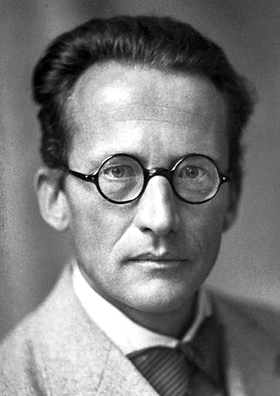
\includegraphics[width=\linewidth]{Schrodinger.jpg}
  \caption{Erwin Schrodinger}
  \label{fig:fig}
\end{marginfigure}
\begin{marginfigure}[30pt]
  
\includegraphics[width=\linewidth]{schrodingers_cat.jpg}
  \caption{Schrodinger's cat}
  \label{fig:fig}
\end{marginfigure}

The Schr�dinger equation is the fundamental equation of physics for describing quantum mechanical behavior. It is also often called the Schr�dinger wave equation, and is a partial differential equation that describes how the wavefunction of a physical system evolves over time. Viewing quantum mechanical systems as solutions to the Schr�dinger equation is sometimes known as the Schr�dinger picture, as distinguished from the matrix mechanical viewpoint, sometimes known as the Heisenberg picture.
$$\mathcal{H}\psi(x,t)=\frac{p^2}{2m}\psi(x,t)+V(x)\psi(x)=E\psi(x,t)$$
$$\frac{-\hbar^2}{2m}\frac{d^2}{dx^2}\psi(x,t)+V(x)\psi(x)=E\psi(x,t)$$
$$\frac{d^2}{dx^2}\psi(x,t)=-\frac{2m}{\hbar^2}\left[E-V(x)\right]\psi(x,t)$$

\section{Uncertainty Relations}
 The uncertainty principle, also known as Heisenberg's uncertainty principle, is any of a variety of mathematical inequalities asserting a fundamental limit to the precision with which certain pairs of physical properties of a particle, known as complementary variables, such as position $x$ and momentum p, can be known simultaneously.  Introduced first in 1927, by the German physicist Werner Heisenberg, it states that the more precisely the position of some particle is determined, the less precisely its momentum can be known, and vice versa
$$(\Delta x)^2=\Braket{x^2}-\Braket{x}^2$$
The uncertainty of a quantity is calculated from the difference between the mean square and the square mean.  The relationship between the uncertainty in position and momentum is as follows.
\marginnote[-80pt]{$$\sigma_x=\Delta x$$
$$\sigma_p=\Delta p$$}
\marginnote[-40pt]{
According to the Copenhagen interpretation, physical systems generally do not have definite properties prior to being measured, and quantum mechanics can only predict the probabilities that measurements will produce certain results. The act of measurement affects the system, causing the set of probabilities to reduce to only one of the possible values immediately after the measurement. This feature is known as wavefunction collapse.\\
Schr�dinger's cat is a thought experiment, sometimes described as a paradox, devised by Austrian physicist Erwin Schr�dinger in 1935. It illustrates what he saw as the problem of the Copenhagen interpretation of quantum mechanics applied to everyday objects. }
$$\Delta x\ \Delta p\geq  \frac{\hbar}{2}$$
The relationship between the uncertainty in energy and time is as follows.
$$\Delta E\ \Delta t\geq \frac{\hbar}{2}$$
As a mathematical system for making statements about the world, quantum mechanics has limits of specificity built in.  These uncertainties are not shortcomings of measurement.  They are hard coded into quantum theory itself.

\section{Particle in a Box}
\begin{marginfigure}[0pt]
  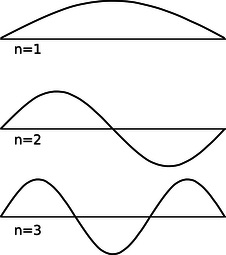
\includegraphics[width=\linewidth]{particle_box.jpg}
  \caption{Particle in a box wavefunctions}
  \label{fig:fig}
\end{marginfigure}

the particle in a box model (also known as the infinite potential well or the infinite square well) describes a particle free to move in a small space surrounded by impenetrable barriers. The model is mainly used as a hypothetical example to illustrate the differences between classical and quantum systems. In classical systems, for example a ball trapped inside a large box, the particle can move at any speed within the box and it is no more likely to be found at one position than another. However, when the well becomes very narrow (on the scale of a few nanometers), quantum effects become important. The particle may only occupy certain positive energy levels. Likewise, it can never have zero energy, meaning that the particle can never "sit still". Additionally, it is more likely to be found at certain positions than at others, depending on its energy level. The particle may never be detected at certain positions, known as spatial nodes.
\marginnote[20pt]{$$\sigma_x^2=\frac{L^2}{12}\left(1-\frac{6}{n^2\pi^2}\right)$$
$$\sigma_p^2=\left(\frac{\hbar n\pi}{L}\right)^2$$
$$\sigma_x \sigma_p = \frac{\hbar}{2} \sqrt{\frac{n^2\pi^2}{3}-2}$$}
$$ \psi(x)=A\sin\left(\frac{n\pi x}{L}\right)$$
$$E_n=\frac{h^2n^2}{8mL^2}$$

\section{Hydrogen Atom and the Bohr Model}
\marginnote{
The principal quantum number (symbolized $n$) is one of four quantum numbers which are assigned to each electron in an atom to describe that electron's state. As a discrete variable, the principal quantum number is always an integer. As $n$ increases, the number of electronic shells increases and the electron spends more time farther from the nucleus. As $n$ increases, the electron is also at a higher potential energy and is therefore less tightly bound to the nucleus.

The principal quantum number was first created for use in the semiclassical Bohr model of the atom, distinguishing between different energy levels. With the development of modern quantum mechanics, the simple Bohr model was replaced with a more complex theory of atomic orbitals. However, modern theory still requires the principal quantum number.
 Apart from the principal quantum number $n$, the other quantum numbers for bound electrons are the azimuthal quantum number $l$, the magnetic quantum number $m$, and the spin quantum number $s$.}

 The 1913 Niels Bohr paper \textit{On the Constitution of Atoms and Molecules} depicts the atom as a small, positively charged nucleus surrounded by electrons that travel in circular orbits around the nucleus.  It is the solar system, but small and attraction provided by electrostatic forces rather than gravity.
 \subsection{Ryberg Formula}
The model's key success lay in explaining the Rydberg formula for the spectral emission lines in of atomic hydrogen.
$$\frac{1}{\lambda} = R\left(\frac{1}{n_1^2}-\frac{1}{n_2^2}\right) $$
The Ryberg constant  $R$ fits the spectral lines of hydrogen with the following value.
$$R=\frac{1.097 \times 10^{7}}{\text{m}}$$
While the Rydberg formula had been known experimentally, it did not gain a theoretical underpinning until the Bohr model was introduced.


\begin{figure*}
  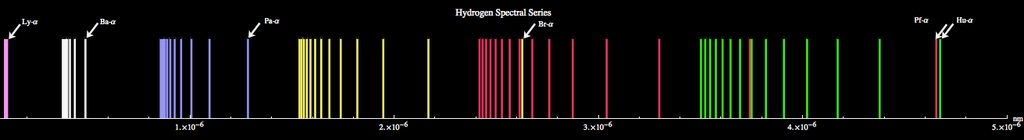
\includegraphics[width=\linewidth]{HydrogenSpectrum.jpg}
  \caption{Hydrogen spectrum}
  \label{fig:fig}
\end{figure*}

\subsection{Quantization of Angular Momentum}
In order to derive the energy levels of the Bohr model begin with quantization of angular momentum.
$$L=n\hbar=mvr$$
This is the quantum fairy dust sprinkled on circular orbits of the electron in a Coulomb field.
\marginnote[-70pt]{\subsection{Coulomb Force}
In this case the Coulomb force provides the centripetal force.
$$F_e=F_c$$
For an electron orbiting a proton the following applies.
$$ \frac{k_ee^2}{r^2}=\frac{m_ev^2}{r}$$
This is useful to parameterize the kinetic energy as a function of radius. 
\subsection{Energy}
Consider the total energy of the hydrogen atom.
$$E=KE+PE$$
$$E=\frac{m_ev^2}{2}-\frac{k_ee^2}{r}$$
Substituting yields a function for the total energy as a function of $r$ or of $v$.
$$E=-\frac{k_ee^2}{2r}=-\frac{m_ev^2}{2}$$
This is used to derive an expression for the radius of orbit $r$ as a function of $v$.
}
\subsection{Orbital Radii}
Applying the quantization of angular momentum yields the following.
$$r= \frac{k_ee^2}{mv^2} \hspace{2cm} v=\frac{n\hbar}{mr}$$
This process identifies the quantized orbital radii of hydrogen.  Remember $n$ is tracking the angular momentum of the hydrogen atom.
$$r_n=\frac{n^2\hbar^2}{m_ek_ee^2}=n^2a_0$$
From the quantized radii the energy levels may be expressed.
$$E_n=-\frac{k_ee^2}{2a_0n^2}=\frac{E_1}{n^2}$$
The wavelength of photon emitted from an electron transition from $m$ to $n$ is written.
$$E_n-E_m=\frac{hc}{\lambda}$$
The Ryberg constant may be identified.
$$R=\frac{E_1}{hc}$$
\marginnote[-80pt]{ \subsection{Quantum Stability}
Experiments by Rutherford in 1909 showed the structure of the atom be a dense, positive nucleus with a light, negative charge orbiting around it. This immediately caused problems on how such a system could be stable. Classical electromagnetism had shown that any accelerating charge radiates energy described through the Larmor formula. If the electron is assumed to orbit in a perfect circle and radiates energy continuously, the electron would spiral into the nucleus.
$$P = {2 \over 3} \frac{q^2 a^2}{  4 \pi \varepsilon_0 c^3}= \frac{q^2 a^2}{6 \pi \varepsilon_0 c^3} \mbox{ (SI units)}$$ 
$$t_\text{fall} \approx \frac{ a_0^3}{4 r_0^2 c} \approx 1.6 \cdot 10^{-11} \text{s}$$}
\section{Schrodinger's Hydrogen}
$$\left(- \frac{\hbar^2}{2 \mu} \nabla^2  - \frac{ Z e^2}{4 \pi \epsilon_0 r} \right) \psi(r,\theta, \phi) = E \psi(r, \theta, \phi)$$
Above is the Schrodinger equation for 3-dimensions.  Expanding in sperical coordinates leaves the following.
\begin{fullwidth}
$$-\frac{\hbar^2}{2 \mu} \left[ \frac{1}{r^2} \frac{\partial }{\partial r} \left( r^2 \frac{ \partial \psi}{\partial r}\right) + \frac{1}{r^2 \sin \theta} \frac{\partial }{\partial \theta} \left( \sin \theta \frac{\partial \psi}{\partial \theta}\right) + \frac{1}{r^2 \sin^2 \theta} \frac{\partial^2 \psi}{\partial \phi^2} \right] - \frac{Z e^2}{ 4 \pi \epsilon_0 r} \psi= E \psi$$
\end{fullwidth}
The solution of the Schr�dinger equation wave equation for the hydrogen atom is written as follows.$$ \psi_{n\ell m}(r,\vartheta,\varphi) = \sqrt {{\left (  \frac{2}{n a_0} \right )}^3 \frac{(n-\ell-1)!}{2n[(n+\ell)!]}} e^{- \rho / 2} \rho^{\ell} L_{n-\ell-1}^{2\ell+1}(\rho) Y_{\ell}^{m}(\vartheta, \varphi ) $$
$$ \rho = {2r \over {na_0}} $$
\begin{marginfigure}
  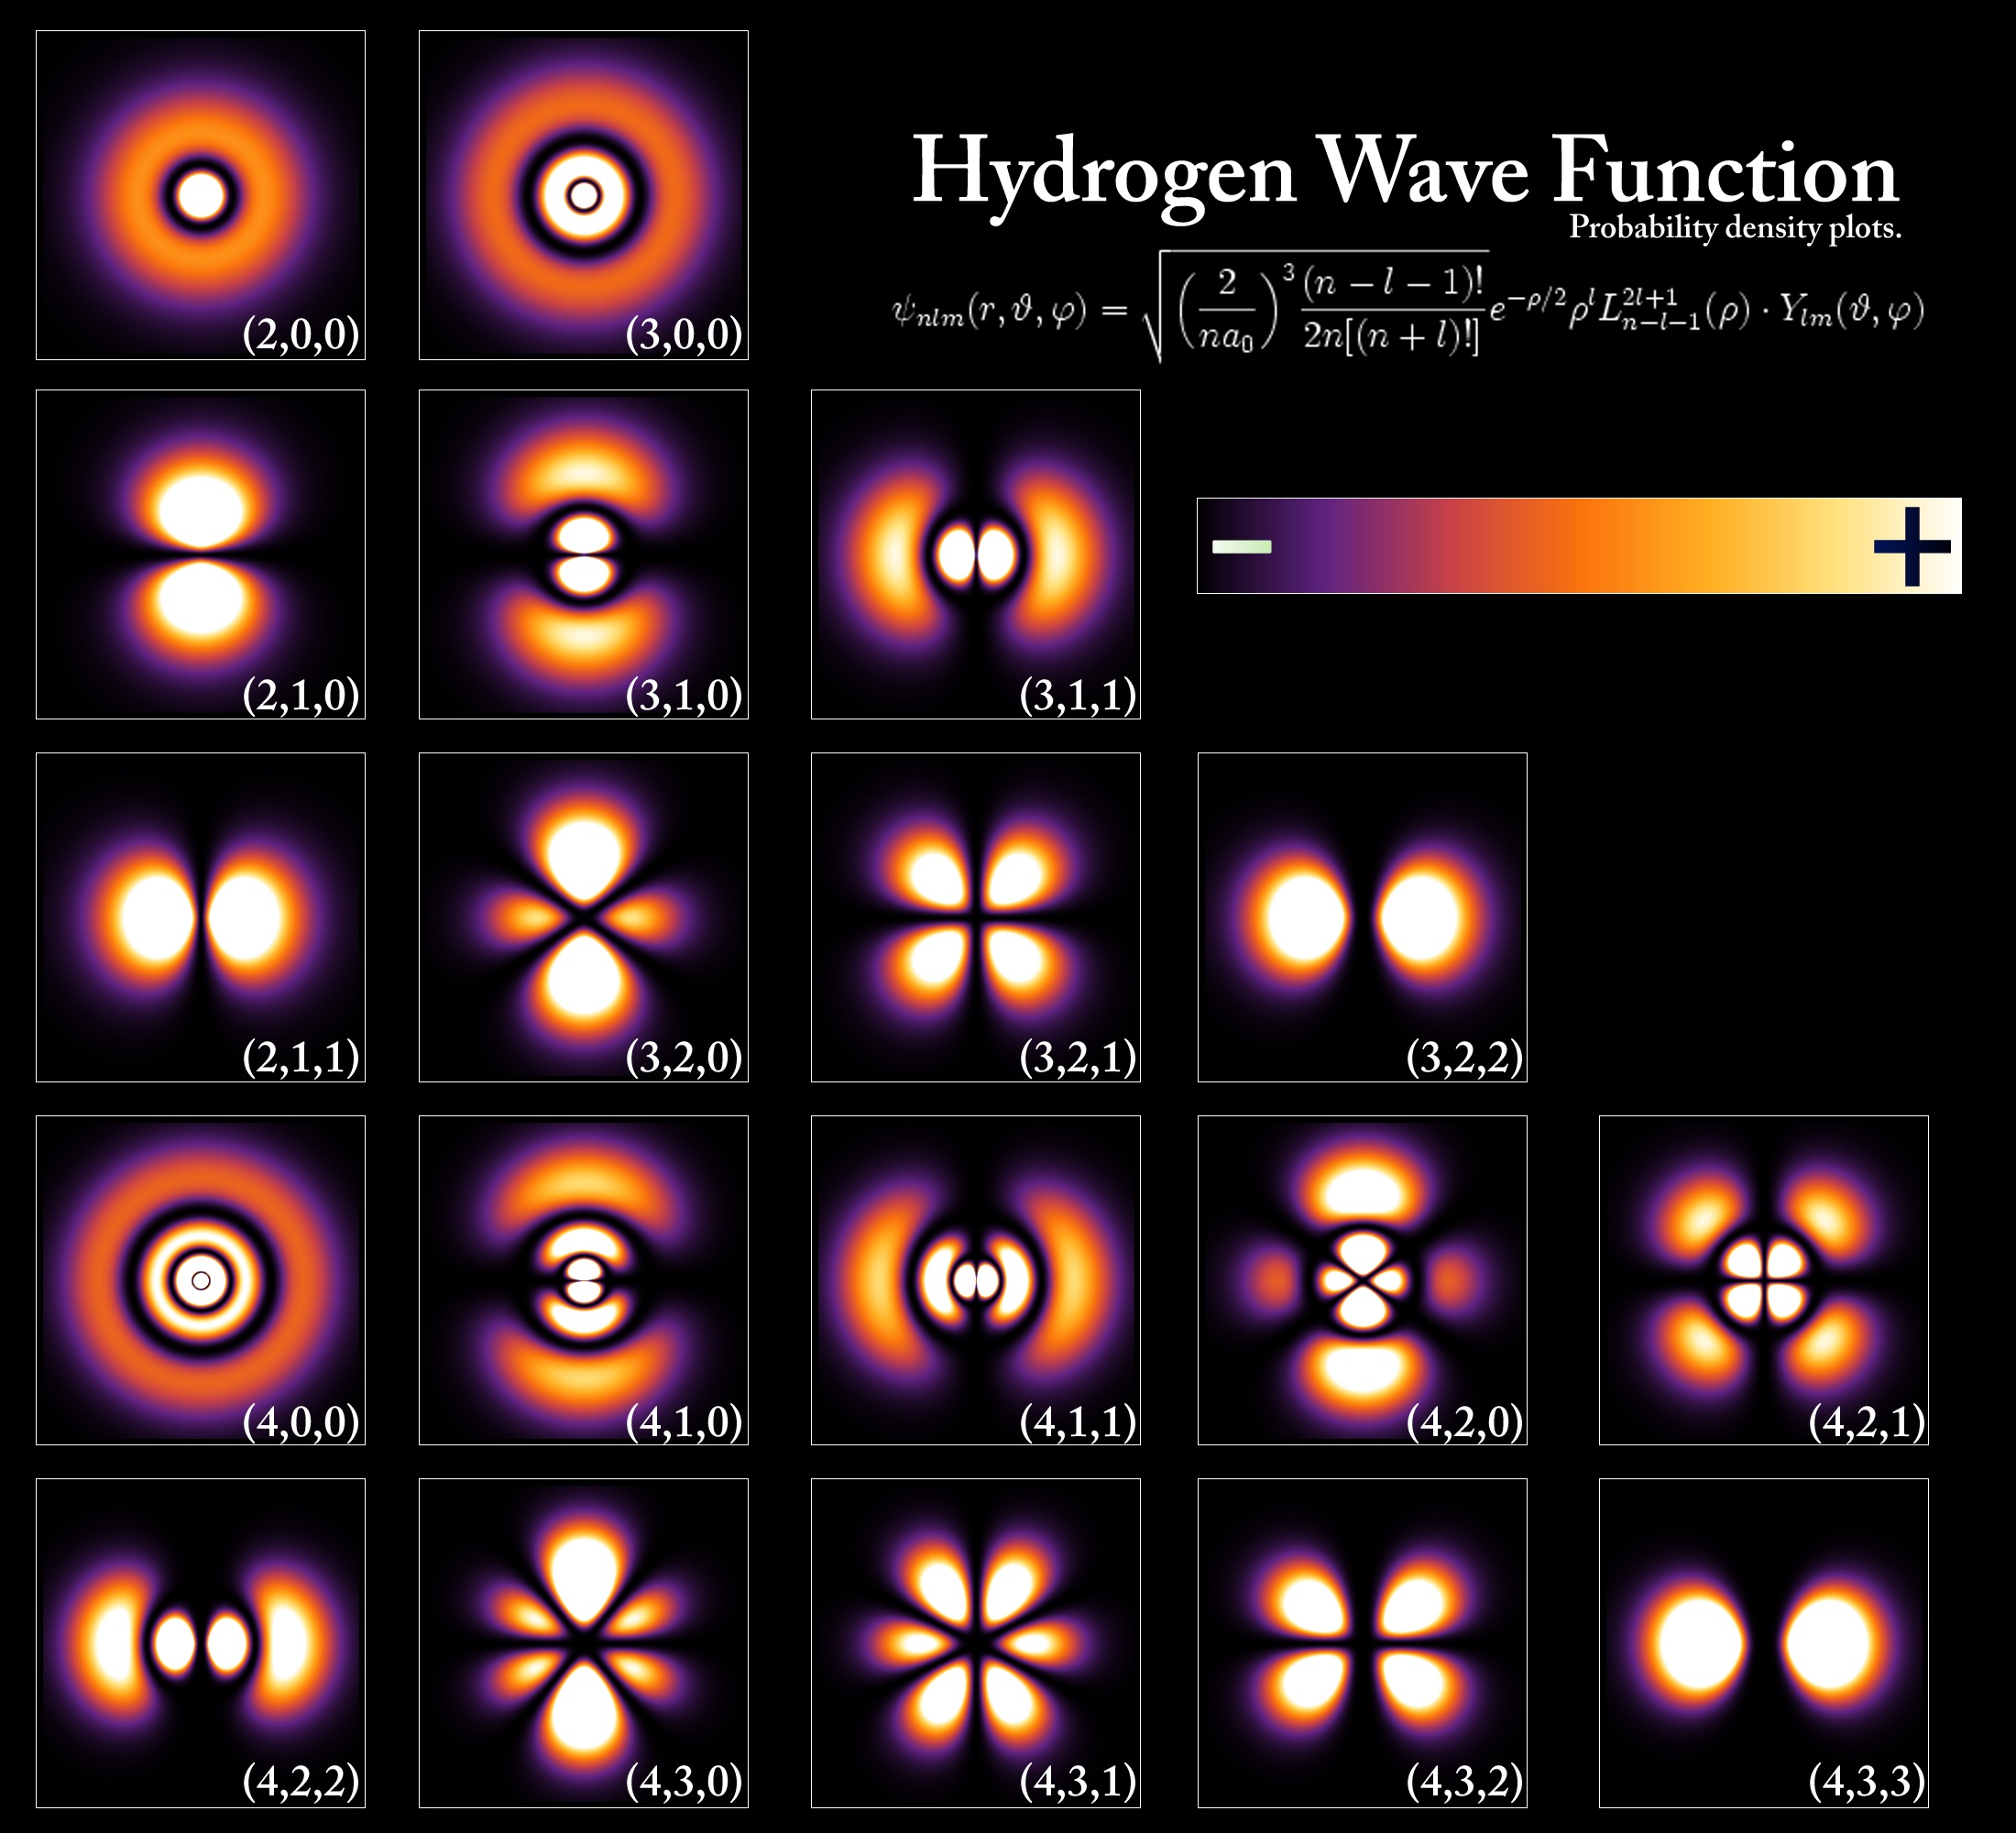
\includegraphics[width=\linewidth]{Hydrogen_Density_Plots.jpg}
  \caption{Hydrogen wave function}
  \label{fig:fig}
\end{marginfigure}
\begin{marginfigure}
  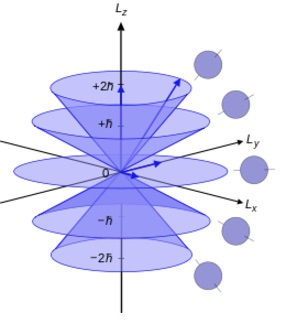
\includegraphics[width=\linewidth]{Lstates.jpg}
  \caption{Quantum numbers $\ell$ and $m$}
  \label{fig:fig}
\end{marginfigure}

$ L_{n-\ell-1}^{2\ell+1}(\rho) $ is the generalized Laguerre polynomial of degree $n-\ell -1$.  Here is a closed form formula.
$$ L_n^{\alpha} (x) = \sum_{i=0}^n (-1)^i {n+\alpha \choose n-i} \frac{x^i}{i!} $$
$Y_{\ell}^{m}(\vartheta, \varphi )$ is the is a spherical harmonic function of degree $\ell$ and order $m$.  Here is a closed form formula.
$$  Y_\ell^m( \theta , \varphi ) = \sqrt{{(2\ell+1)\over 4\pi}{(\ell-m)!\over (\ell+m)!}}  \, P_\ell^m ( \cos{\theta} ) \, e^{i m \varphi } $$
Here $ P_\ell^{m}(x)$ is the associated Legendre polynomial of degree $\ell$ and order $m$.  Here is the Rodriguez formula.
$$ P_\ell^{m}(x) = \frac{(-1)^m}{2^\ell \ell!} (1-x^2)^{m/2}\  \frac{d^{\ell+m}}{dx^{\ell+m}}(x^2-1)^\ell$$


The energy eigenstates may be classified by two angular momentum quantum numbers, $\ell$ and m (both are integers). The angular momentum quantum number $\ell = 0, 1, 2, ...$ determines the magnitude of the angular momentum. The magnetic quantum number $m = -\ell, ..., +\ell$ determines the projection of the angular momentum on the (arbitrarily chosen) z-axis.

The Schrodinger hydrogen is a probability distribution. The ground state is spherically symmetric, in fact all $\ell=0$ states are symmetric.  The average radial position of these probability distribution functions corresponds to the quantized radii of the Bohr atom.
\begin{marginfigure}
  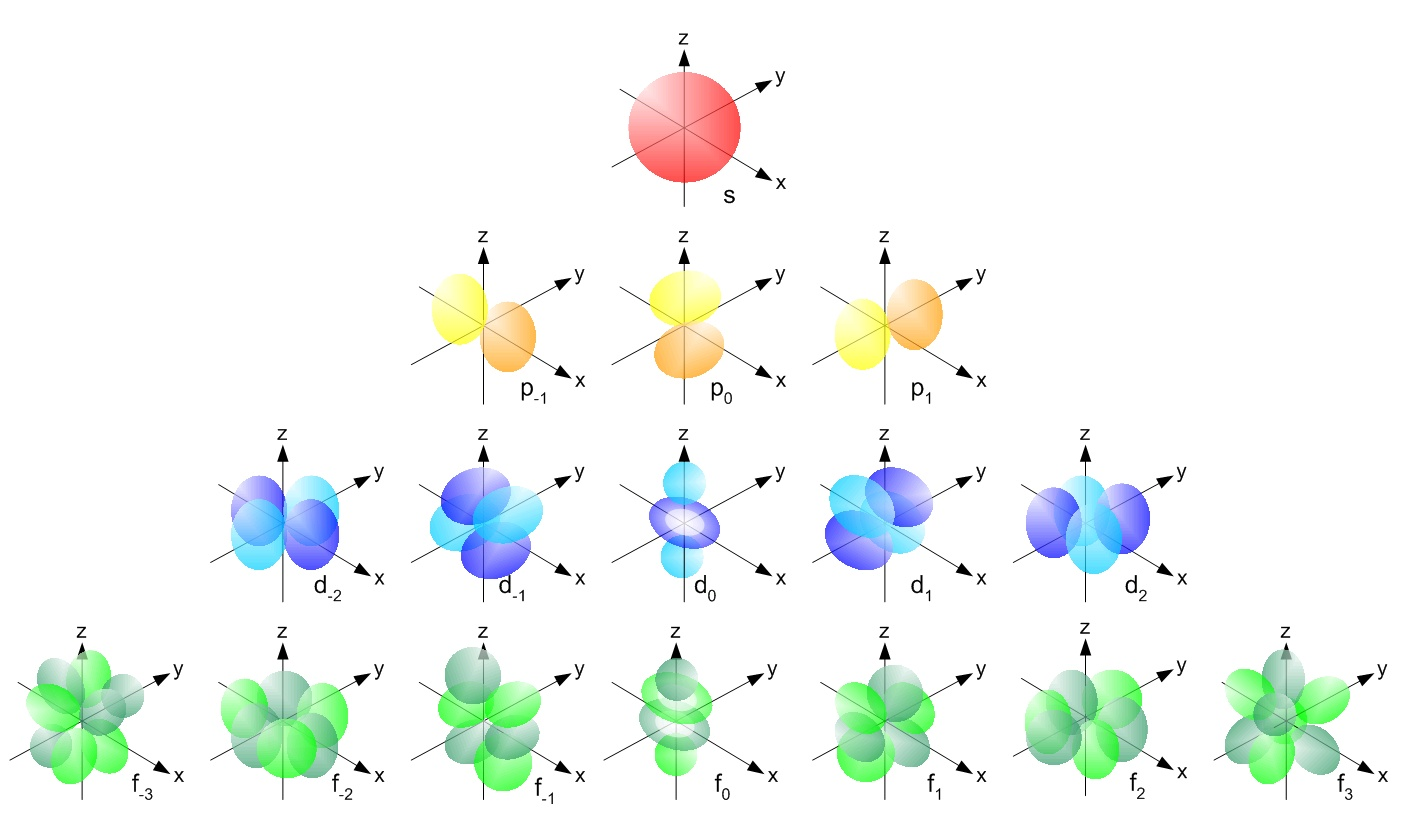
\includegraphics[width=\linewidth]{orbs.jpg}
  \caption{Spherical harmonics}
  \label{fig:fig}
\end{marginfigure}
$$\braket{r}_{n}=n^2a_0$$
Note the $\ell=0$ states correspond to zero angular momentum.  Compare this to the Bohr model ground state.
\section{Harmonic Oscillator}
The quantum harmonic oscillator is the quantum-mechanical analog of the classical harmonic oscillator. Because an arbitrary potential can usually be approximated as a harmonic potential at the vicinity of a stable equilibrium point, it is one of the most important model systems in quantum mechanics. Furthermore, it is one of the few quantum-mechanical systems for which an exact, analytical solution is known.
\marginnote[-80pt]{
$$V(x)=\frac{kx^2}{2}=\frac{m\omega^2x^2}{2}$$
$$E=\frac{m\omega^2A^2}{2}$$
\subsection{Ground State Wavefunction}
$$\psi_0(x)=Be^{-Cx^2}$$
$$C=\frac{m\omega}{2\hbar} \hspace{2cm} E_0=\frac{\hbar \omega}{2}$$

}
$$\frac{d^2}{dx^2}\psi(x)=-\frac{2m}{\hbar^2}\left[E-\frac{m\omega^2x^2}{2}\right]\psi(x)=-\left[\frac{2mE}{\hbar^2}-\left(\frac{m\omega}{\hbar}\right)^2x^2\right]\psi(x)$$

\subsection{Quantized Energy States}
$$E_{n+1}-E_n=\hbar \omega$$
From the ground state it is possible to ladder up the states.  This is the general solution of the wavefunction.
\begin{marginfigure}
  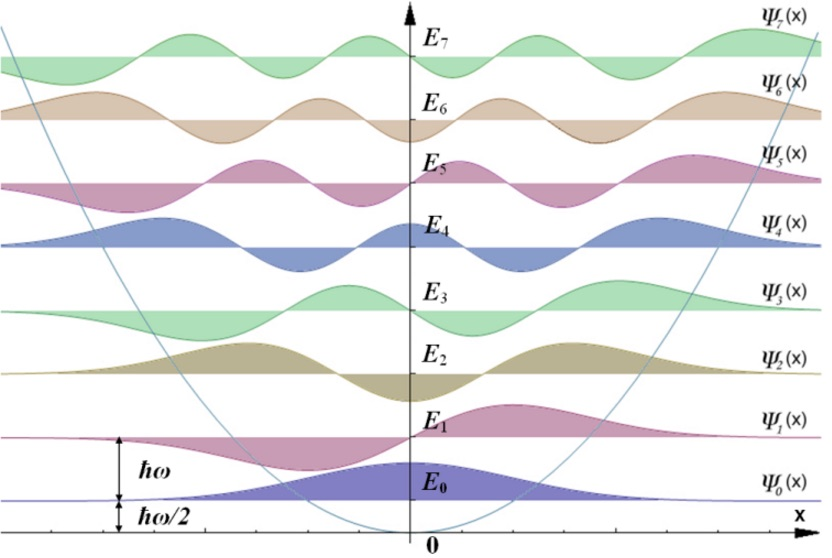
\includegraphics[width=\linewidth]{harmosc.jpg}
  \caption{Quantized harmonic oscillator}
  \label{fig:fig}
\end{marginfigure}
\begin{marginfigure}
  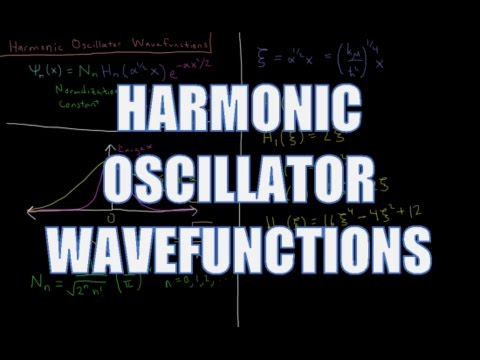
\includegraphics[width=\linewidth]{howave.jpg}
  \caption{Harmonic oscillator wavefunctions}
  \label{fig:fig}
\end{marginfigure}
\begin{marginfigure}
  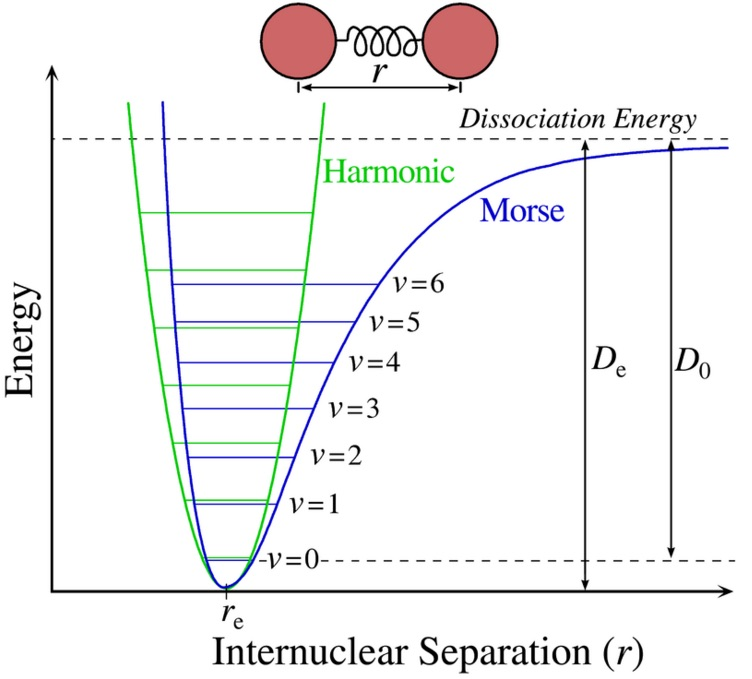
\includegraphics[width=\linewidth]{harmo.jpg}
  \caption{Harmonic approximation}
  \label{fig:fig}
\end{marginfigure}
$$  \psi_n(x) = \frac{1}{\sqrt{2^n\,n!}} \cdot \left(\frac{m\omega}{\pi \hbar}\right)^{1/4} \cdot e^{
- \frac{m\omega x^2}{2 \hbar}} \cdot H_n\left(\sqrt{\frac{m\omega}{\hbar}} x \right), \qquad n = 0,1,2,\ldots$$
Where $H_n$ are Hermite polynomials.  The Rodriquez formula is written below.
$$H_n(z)=(-1)^n~ e^{z^2}\frac{d^n}{dz^n}\left(e^{-z^2}\right)$$
The quantized energy states are written as follows.
$$ E_n = \hbar \omega \left(n + {1\over 2}\right) = (2 n + 1) {\hbar \over 2} \omega$$
This energy spectrum is noteworthy for three reasons. First, the energies are quantized, meaning that only discrete energy values.  Second, these discrete energy levels are equally spaced, unlike in the Bohr model of the atom, or the particle in a box. Third, the lowest achievable energy (the energy of the n = 0 state, called the ground state) is not equal to the minimum of the potential well, but $\nicefrac{\hbar \omega}{2}$ above it; this is called zero-point energy. Because of the zero-point energy, the position and momentum of the oscillator in the ground state are not fixed (as they would be in a classical oscillator), but have a small range of variance, in accordance with the Heisenberg uncertainty principle. This zero-point energy further has important implications in quantum field theory and quantum gravity.



